\documentclass[oneside]{homework} %%Change `twoside' to `oneside' if you are printing only on the one side of each sheet.
\usepackage{amsmath}
\usepackage{amssymb,mathtools}
\usepackage{graphicx}
\graphicspath{}

\studname{Alex Wong}
\studmail{asw2181@columbia.edu}
\coursename{COMS E6232}
\hwNo{3}
\uni{asw2181}

\begin{document}
\maketitle
\skipevenpage

\problemNo{1}
{\large a.} Consider an instance where we have two items x and y where $s_x = \epsilon$, $v_x = 2\epsilon$, $s_y = B$, $v_y =B$, and $\epsilon << 1$. The $v_i/s_i$ ratio of item x is 2 and item y is 1. Thus, the Greedy algorithm will always pick item x regardless of how large B is and regardless how small $\epsilon$ is. So as B gets larger and/or $\epsilon$ gets smaller, the approximation ratio of the algorithm will increase, thus showing that the approximation ratio of Greedy is not bounded by any constant. \hfill\qed
\newline
\newline
{\large b.} \textbf{Theorem 1b} The Modified Greedy algorithm achieves approximation ratio 2.
\newline

\textbf{Proof:} Let $OPT$ be the optimal solution that has maximum value where $v(OPT) = \sum\limits_{i\epsilon OPT}v_i$ subject to $\sum\limits_{i\epsilon OPT}s_i \leq B$. We first assume that the items are ordered in a non-increasing fashion according to the ratio $v_i/s_i$. Let's call the first item that does not fit in the knapsack using the Greedy algorithm as item $m$. We know that item $m$'s $v_i/s_i$ ratio $\geq$ items $m+1,...,n$'s $v_i/s_i$ ratio. Thus, if we are able to fit some fraction of item $m$ so that it fills up to the capacity of the knapsack, that solution will be $\geq$ OPT. We can define the fraction of item $m$ that fits into the knapsack as $\alpha$ where $\alpha = (B - \sum\limits_{i=1}^{m-1} v_i) / s_m$. Thus, $OPT \leq (\sum\limits_{i=1}^{m-1} v_i) + \alpha v_m$. Since $\alpha$ is some fraction $\leq 1$, we can also say that: $$OPT \leq (\sum\limits_{i=1}^{m-1} v_i) + \alpha v_m \leq (\sum\limits_{i=1}^{m-1} v_i) + v_m$$ From the inequality above, $\sum\limits_{i=1}^{m-1} v_i$ or $v_m$ must be at least $OPT/2$, showing that the Modified Greedy algorithm will always get a solution at least $OPT/2$, thus achieving an approximation ratio 2. \hfill\qed

\problemNo{2}
{\large a.} The lower bound for OPT is $max(max_i(p_i), \frac{\sum\limits_{i=1}^{n}p_i}{m})$. 
\newline
\newline
For $m$ = 2 machines and 5 jobs with processing times 3,3,2,2,2, the LPT algorithm will schedule 3,2,2 on $m_1$ and 3,2 on $m_2$, giving a makespan of 7. For OPT, we know that a lower bound is max = $max(3, 12/2) = 6$. We can achieve OPT by scheduling 2,2,2 on one machine and 3,3 on the other machine.
\newline
\newline
For $m$ = 3 machines and 7 jobs with processing times 5,5,4,4,3,3,3, the LPT algorithm will schedule 5,3,3 on $m_1$, 5,3 on $m_2$, and 4,4 on $m_3$, giving a makespan of 11. For OPT, the lower bound is $max(5, 27/3) = 9$. We can achieve OPT by scheduling 3,3,3 on one machine and 5,4 on each of the other two machines.
\newline
\newline
{\large b.} If $p_n > OPT/3$, then $3p_n > OPT$, showing that no machine can process more than 2 jobs or else it would be $>$ OPT, which would contradict OPT being the optimal solution. From this, we know that $n \leq 2m$, thus the largest $m$ jobs will first get scheduled on each of the $m$ machines and the rest of the $n - m$ jobs will be assigned to the machine that has the least load at the point of assignment, thus showing that the LPT schedule is optimal. \hfill\qed
\newline
\newline
{\large c.} \textbf{Theorem 2c} LPT achieves an approximation ratio of 4/3.
\newline

\textbf{Proof:} Let's define job $j$ as the job that finishes last in the LPT schedule and $t_j$ as the span of time from time 0 until the time that job $j$ starts. We know that in the timespan of $t_j$, $m\cdot t_j$ amount of processing has been done. This amount of processing can't be more than the total amount of processing of all jobs, thus $m \cdot t_j \leq \sum\limits_{i=1}^{n}p_i \implies t_j \leq \frac{\sum\limits_{i=1}^{n}p_i}{m}$. As we saw earlier in part $a$, $\frac{\sum\limits_{i=1}^{n}p_i}{m}$ is essentially a lower bound for OPT, thus we can say that $t_j \leq OPT$. Then by adding $p_j$ to $t_j$, we get the makespan of the machine that has scheduled job $j$, and we can say that $t_j + p_j \leq OPT + p_j$. What the inequality tells us is that the processing time of job $j$ indicates how well the LPT algorithm performs. Referring to part $b$, if $p_j > OPT/3$, the LPT schedule is optimal. But in the worst case, if $p_j = OPT/3$, then LPT will give an $OPT + p_j = OPT + OPT/3 = 4/3 OPT$ makespan, thus showing that LPT achieves an approximation ratio of 4/3. \hfill\qed
\newline
\newline
{\large d.} \textbf{Theorem 2d} The ratio of 4/3 of LPT is asymptotically tight as $m \rightarrow \infty$.
\newline

\textbf{Proof:} We generalize the examples of part $a$: given $m$ machines, we have 3 jobs that have a processing time of $m$, and 2 jobs for each processing time $2m-1,...,m+1$ (if $2m-1 = m+1$, then there are only 2 jobs for both $2m-1$ and $m+1$) giving us a total of 2m+1 jobs. With LPT scheduling, we find that every machine will get scheduled two jobs with a total processing time of $3m-1$ with exception of the first machine that will get scheduled with 3 jobs with a total processing time of $3m-1+m = 4m-1$. Thus, the makespan with LPT scheduling is $4m-1$. For an optimal makespan $OPT$, we first schedule all 3 jobs with processing time $m$ on the first machine, and then use LPT scheduling for the rest of the jobs. This will give each machine a total processing time of $3m$, thus making the makespan of $OPT = 3m$. Without loss of generality, the figure below illustrates the makespan of LPT and $OPT$ of the example from part $a$ when $m = 3$:
\begin{figure}[h]
\centering
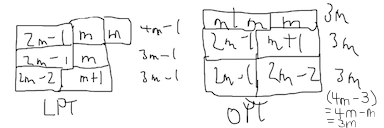
\includegraphics{2d1}
\caption{Makespan of LPT = 4m - 1, Makespan of OPT = 3m}
\end{figure}
\newline
Thus, we see the ratio of $LPT/OPT = (4m - 1) / 3m = \frac{4m}{3m} - \frac{1}{3m} = \frac{4}{3} - \frac{1}{3m}$, showing that the approximation ratio 4/3 is asymptotically tight as $m \rightarrow \infty$. \hfill\qed

\problemNo{3}
{\large a.} \textbf{Lemma 3a} If $I$ is an independent set of $G$ then $I^k$ is an independent set of $G^{(k)}$.
\newline

\textbf{Proof:} For $I$ to be an independent set of $G$, there must be no adjacent edges between any of the nodes of $I$. Given the definition of $E^{(k)}$ of $G^{(k)}$, $$E^{(k)} = \{(u, v) \in N^{(k)} \times N^{(k)} \mid \exists i, j \in [k], (u_i, u_j) \in E \text{ or } (v_i, v_j) \in E \text{ or } (u_i, v_j) \in E\}$$ we can see that there are no edges between any pairs $(u, v)$ of $k$-tuples of nodes that only contain nodes of $I$. When taking the Cartesian product of $I$, $I^k$, we create $k$-tuples using only those nodes from $I$ so $I^k \subseteq N^{(k)}$ since $I \subseteq N$. Also, as explained earlier, the $k$-tuples of $I^k$ do not have adjacent edges between them since they only contain nodes of $I$, thus showing that $I^k$ is an independent set of $G^{(k)}$. \hfill\qed
\newline
\newline
{\large b.} \textbf{Lemma 3b} If $J$ is an independent set of $G^{(k)}$ then we can construct in polynomial time an independent set $I$ of $G$ of size at least $|J|^{1/k}$ and conclude that $\alpha(G^{(k)}) = (\alpha(G))^k$
\newline

\textbf{Proof:} From Lemma 3a, if $I$ is an independent set of $G$, then $I^k$ is an independent set of $G^{(k)}$. Since we have defined $J$ to be an independent set of $G^{(k)}$, we can use Lemma 3a to say that $J = I^k$. The size of $J$ is then equal to the size of $I^k$, which is $|I|^k$, thus $|J| = |I|^k \Longrightarrow |I| = |J|^{1/k}$, showing that we can construct in polynomial time an independent set $I$ of $G$ of size at least $|J|^{1/k}$. Also, if given the maximum independent set of $G$, $\alpha(G)$, we can use our earlier conclusion and see that $(\alpha(G^{(k)}))^{1/k} = \alpha(G) \Longrightarrow \alpha(G^{(k)}) = (\alpha(G))^k$. \hfill\qed
\newline
\newline
{\large c.} \textbf{Lemma 3c} If the Maximum Independent Set problem can be approximated in polynomial time within some constant factor $c > 1$, then it has a PTAS.
\newline

\textbf{Proof:} We first define $\alpha(G)$ as the maximum independent set of $G$. From the PCP theorem, we can trivially say that the Maximum Independent Set problem has a 2-approximation algorithm. Let us define $I$ as an independent set of G that agrees with the 2-approximation algorithm. This means that the size of $I$ will be $1/2$ the size of the maximum independent set of $G$, thus $\frac{|\alpha(G)|}{|I|} = 2$. Now, using Lemma 3b, if we take the $k$-th power of the graph G, we know that $\alpha(G^{(k)}) = (\alpha(G))^k$ and by Lemma 3a, $I^k$ is an independent set of $G^{(k)}$. Thus, for some $k$-th power graph $G^{(k)}$, the approximation ratio is $\frac{|\alpha(G)|^k}{|I|^k} = (\frac{|\alpha(G)|}{|I|})^k = 2^k$ which shows that the approximation ratio grows as we apply the approximation algorithm to larger and larger $k$-th powers of graph $G$. Thus, the Maximum Independent Set problem can not be approximated in polynomial time within some constant factor, which means it does not have a PTAS unless \textbf{P = NP}. \hfill\qed

\problemNo{4}
{\large a.} \textbf{Lemma 4a} MDAS can be trivially approximated within a factor of 2.
\newline

\textbf{Proof:} Suppose we have an arbitrary ordering of nodes $v_1, ..., v_n$ and we have two subsets of edges $A_1$ and $A_2$ where $$A_1 = \{(v_i, v_j) \mid (v_i, v_j) \in A, i < j\}$$ $$A_2 = \{(v_i, v_j) \mid (v_i, v_j) \in A, i > j\}$$ By separating the edges into these two subsets, the only way for $A_1$ to contain a cycle is if there is an edge where $i > j$, which would be contained in the $A_2$ subset, and the only way for $A_2$ to contain a cycle is if there is an edge where $ i < j$, which would be contained in the $A_1$ subset. Thus, neither subset will contain a cycle and at least one of the two subsets will contain at least $|A|/2$ edges since $A = A_1 + A_2$. Thus, MDAS can be trivially approximated within a factor of 2 by taking the larger of the two subsets. \hfill\qed
\newline
\newline
{\large b.} \textbf{Theorem 4.2} The Maximum Directed Acyclic Subgraph (MDAS) problem does not have a PTAS unless \textbf{P = NP}.
\newline

\textbf{Proof:} A known problem that does not have a PTAS is the Maximum Independent Set (MIS) problem. MIS does not have a PTAS for any graph with a maximum degree $\geq 3$. We can do a linear reduction $MIS(3) \leq_L MDAS$: Given an undirected graph $G = (N, E)$ with maximum degree 3, we construct a directed graph $D = (V, A)$ where $V = \{(u_1, u_2) \mid u \in N\}$ and $A = \{(u_1, u_2) \mid u \in N\}  \cup \{(u_2, v_1),(v_2, u_1) \mid (u, v) \in E\}$. We let $\alpha(G)$ denote the size of the maximum independent set of $G$ and $\gamma(D)$ denote the number of edges of the maximum acyclic subgraph of $D$. From this, we have the following lemma:
\newline

\textbf{Lemma 4.2.1} For all $\epsilon > 0$, if we are given an acyclic subgraph of $D$ that has at least $(1-(\epsilon/13))\gamma(D)$ edges, then we can compute in polynomial time an independent set $G$ that has at least $(1-\epsilon)\alpha(G)$ nodes.
\newline

\textbf{Proof}:
\newline
\textbf{(4.2a)} If $I$ is an independent set of $G$, then $D' = (V, A')$ where $A' = \{(u_1, u_2) \mid u \in I\} \cup \{(u_2, v_1), (v_2, u_1) \mid (u, v) \in E\}$ is an acyclic subgraph of $D$. We can see that all edges $\{(u_2, v_1), (v_2, u_1) \mid (u, v) \in E\}$ do not create a cycle because as we have shown in Lemma 4a, a set of edges $\{(v_i, v_j) \mid (v_i, v_j) \in A, i > j\}$ do not create a cycle. We also know that the independent set $I$ contains nodes that do not have any adjacent edges with each other. Thus, since $A'$ contains all the linear reduction of edges of $E$, the only way to keep the edge set acyclic would be to only add the edges $\{(u_1, u_2) \mid u \in N\}$ where the nodes do not have any adjacent edges, which would be the independent set $I$ and gives us $\{(u_1, u_2) \mid u \in I\}$. Thus, if $I$ is an independent set of $G$, then $A'$ is an acyclic subgraph of $D$.
\newline
\newline
\textbf{(4.2b)} Now we show that if $H$ is an acyclic subgraph of $D$ with $h$ edges, we can then derive efficiently from $H$ an independent set of $G$ with at least $h-2|E|$ nodes. As we have shown in \textbf{4.2a}, acyclic subgraphs of $D$ includes all edges $\{(u_2, v_1), (v_2, u_1) \mid (u, v) \in E\}$.  We can see that each edge of $E$ corresponds to two edges in $A$. If we took away all those edges from $H$, we would be left with edges $\{(u_1, u_2) \mid u \in N\}$ which we know are nodes that could create an independent set, as we have shown in \textbf{4.2a}. Thus, we can derive efficiently from $H$ an independent set of $G$ with at least $h-2|E|$ nodes.
\newline
\newline
\textbf{(4.2c)} Lastly, since $G$ has maximum degree 3, we can show that $\alpha(G) \geq |E|/6$. Without loss of generality, lets take a node $u \in N$ that has degree 3, which would imply 4 connected nodes. If we were to make all these nodes connected together, we would have a complete graph where each of the 4 nodes would have a maximum degree of 3. This complete graph has a 6 total edges. From this complete graph, we can only choose any one node as the maximum independent set $\alpha(G)$ as all nodes are adjacent to all other nodes. Thus, we can see that $\alpha(G) \geq |E|/6$.
\newline
\newline
Let us do the linear reduction from MIS to MDAS. From \textbf{4.2b} we know we can get an acyclic subgraph of $D$ with $|I| + 2|E|$ edges. If $I = \alpha(G)$, then getting an acyclic subgraph $D$ with $\alpha(G) + 2|E|$ would imply a maximum acyclic subgraph $\gamma(D)$. We can manipulate our conclusion from \textbf{4.2c} where $\alpha(G) \geq |E|/6 \Longrightarrow |E| \leq 6\cdot\alpha(G)$. Thus, we can say $$\gamma(D) = \alpha(G) + 2|E| \leq \alpha(G) + 12\cdot\alpha(G) = 13\cdot\alpha(G)$$ Based on this L-reduction, it satisfies the first property that $OPT_{MDAS} \leq \alpha \cdot OPT_{MIS}$ where $\alpha = 13$. We can also see it satisfies the second property $|C_1 - OPT_{MIS}| = \beta\cdot|C_2 - OPT_{MDAS}|$ where $\beta = 1$. Combining both properties, we get the relative error: $$\frac{|C_1 - OPT_{MIS}|}{OPT_{MIS}} \leq \frac{\alpha\cdot\beta\cdot|C_2 - OPT_{MDAS}|}{OPT_{MDAS}} \leq \alpha\beta\epsilon$$ Showing that the relative error of MIS is $13\cdot \epsilon$ in relation to the relative error of MDAS being $\epsilon$. Thus, if we wanted to express the relative error of MIS as just $\epsilon$, that would mean that the relative error of MDAS would be $\epsilon/13$. Thus for all $\epsilon > 0$, if we are given an acyclic subgraph of $D$ that has at least $(1-(\epsilon/13))\gamma(D)$ edges, then we can compute in polynomial time an independent set $G$ that has at least $(1-\epsilon)\alpha(G)$ nodes, which proves the lemma. \hfill\qed
\newline
\newline
But because MIS does not have a PTAS as we have proven in problem 3, and since $MIS \leq_L MDAS$, that tells us that MDAS also does not have a PTAS unless \textbf{P = NP}, thus the theorem is proved. \hfill\qed


\end{document}